\documentclass{beamer}
\usetheme{Boadilla}
\title{An application of the Markov Chains in Digital Communication}
\author{Parvez Alam: AI21RESCH01005}
\institute{Indian Institute of Technology \\ Hyderabad}
\date{\today}
\usepackage{tikz}
\usetikzlibrary{automata,positioning}
\usepackage{amsmath}
\begin{document}
\begin{frame}
\titlepage    
\end{frame}

\begin{frame}
\begin{block}{Abstract}
\begin{itemize}
    \item This contribution shows an application of Markov chains in digital communication.
    \item A random sequence of the symbols 0 and 1 is analyzed by a state machine.
    \item The state machine switches to state “0” after detecting an unbroken sequence of w zero symbols (w being a fixed integer), and to state “1” after detecting an unbroken sequence of w ones.
    \item The task to find the probabilities of each of these two states after n time steps leads to a Markov chain.
    \item We show the construction of the transition matrix and determine the steady-state probabilities for the time-homogeneous case.
\end {itemize}
    
\end{block}
    
\end{frame}

\begin{frame}
  \begin{block}{Markov Chain}
  \begin{itemize}
    \item Let \(X_n\) be a random variable that characterizes the state of the studied system at discrete points in time n = 0, 1, 2, . . . The family of random variables {\(X_n\)} forms a stochastic process. This stochastic process is called a Markov process.
 if the occurrence of a future state depends only on the immediately preceding state, i.e., if
  \begin{align}
      \Pr(X_{n+1}=x_{n+1}|X_n=x_n, X_{n-1}=x_{n-1},.......,X_2=x_2,X_1=x_1)\nonumber\\=\Pr(X_{n+1}=x_{n+1}|X_n=x_n) \nonumber
  \end{align}
  \item Let \(p_{ij}\)(n) is the probability of moving from state i at time n to state j at time n+1, then
  \begin{align}
      p_{ij}(n) &=\Pr(X_{n+1}=j|X_n=i),\hspace{0.5cm} i,j=1,2,3,....m \nonumber
  \end{align}
  \end{itemize}
    
  \end{block}
    
\end{frame}
\begin{frame}
   \begin{block}{Continue...}
   \begin{itemize}
      \item The transition matrix is defined as :
    \begin{align}
        \textbf{P}(n)&=\begin{pmatrix}
                       p_{11} & p_{12} & p_{13} & ......& p_{1m} \\
                       p_{21} & p_{22} & p_{23} & ......& P_{2m}\\
                       p_{31} & P_{32} & P_{33} & ......& p_{3m}\\
                       ....&.....&....&..........&....\\
                       p_{m1} & p_{m2} & p_{m3} & ......& p_{mm}
                       \end{pmatrix} \nonumber
    \end{align}
    \item Let define
    \begin{align}
        a_{j}(n)=\Pr(X_n=j),\hspace{0.5cm} j=1,2,3,,m,\hspace{0.5cm} n=0,1,2,3,4,.... \nonumber
    \end{align}
    Given the initial probabilities  \(\textbf{a}(0)=(a_{1}(0),a_{2}(0),a_{3}(0),......,a_{m}(0))\) and the transition matrix \textbf{P}(n) the probabilities  \(\textbf{a}(n)=(a_{1}(n),a_{2}(n),a_{3}(n),......,a_{m}(n))\) is computed as follows:
    \begin{align}
    \textbf{a}(1)&=\textbf{a}(0)\textbf{P}(0) \nonumber \\
    \textbf{a}(2)&=\textbf{a}(1)\textbf{P}(1)=\textbf{a}(0)\textbf{P}(0)\textbf{P}(1) \nonumber
    \end{align}
    \end{itemize}
   \end{block}
    
\end{frame}
\begin{frame}
  \begin{block}{Continue...}
  and recursively
  \begin{align}
      \textbf{a}(n)&=\textbf{a}(0)\prod_{k=0}^n\textbf{P}(k) \hspace{0.5cm} n=1,2,3,4,5,6,....\nonumber
  \end{align}
    
  \end{block}
    
\end{frame}

\begin{frame}
\begin{block}{Formulation of the problems}
\begin{itemize}
 \item A random sequence of 0's and 1's is analysed.The state machine switches to state “0” after detecting an unbroken sequence of w zero symbols, and to state “1” after detecting an unbroken sequence of w ones. Let the random variables  \(X_n\), n = 0, 1, 2, . . .  denotes this process. In this case, \(X_n\) can assume only the values 0 and 1.\\
 \item Denote the probability of state "0" after n time step as x(n):
 \begin{align}
    x(n) &=\Pr(X_n=0) \nonumber
 \end{align}
 \item Denote the probability of state "1" after n time step as y(n):
 \begin{align}
    y(n)&=\Pr(X_n=1) \nonumber
 \end{align}
 \item For determining the x(n) and y(n) a markov chain can be used 
 \begin{center}
   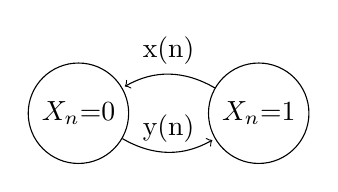
\begin{tikzpicture}
      \node[state] (0) {\(X_n\)=0};
      \node[state, right = of 0] (1) {\(X_n\)=1};
      \draw[every loop]
      (0) edge[bend right,auto=left] node {y(n)} (1)
      (1) edge[bend right,auto=right] node {x(n)} (0);
   \end{tikzpicture}
 \end{center}
\end{itemize}
\end{block}
\end{frame}
\begin{frame}
   \begin{block}{Construction of the transition matrix}
   \begin{itemize}
   \item Unfortunately, we cannot use the Markov chains directly for computing the desired probabilities x(n) and y(n). This is because the fact that if, e.g., the current state of the system is “0”, then the probability that it will become “1” in the next time step depends upon various factors, not only on the current state and the last symbol in the random sequence \(R_n\).Let us explain it on the example of w = 3, i.e., on the case where the state switches after the occurrence of 3 equal symbols.
    \begin{example}
       In this case, if the state at time n was “1” and at time n + 1 it has
       become “0” (which means that the end of the determining sequence of symbols
       is . . . , 0, 0, 0), then it cannot return to state “1” at times n + 2 and n + 3, but
       first at time n + 4. Thus, markov property does not hold here.
    \end{example}
    \item It shows that to overcome this problem, it is convenient to consider more states than just only “0” and “1”. 
   \end{itemize}
   \end{block}
    
\end{frame}
\begin{frame}
  \begin{block}{continue...}
  \begin{itemize}
  \item We will take into account how close to switching the situation is, i.e., how long the unbroken line of ones (if the current state is “0”) or the unbroken line of zeros (if the current state is “1”) is.
  \item  Let us define new random variable\(Y_n\) with 2w possible values as follows:\\
   \(Y_n\) = 1 (state “0-0”) if \(X_n\) = 0 and the last symbol that came is 0,\\
   \(Y_n\) = 2 (state “0-01”) if \(X_n\) = 0 and the last two symbols are 0, 1, \\
   \(Y_n\) = 3 (state “0-011”) if \(X_n\) = 0 and the last three symbols are 0, 1, 1, \\
   ...\\
   ...\\
   ...\\
   ...\\
   \(Y_n\) = w (state “0-011 . . . 1”)(w-1 1's) if \(X_n\) = 0 and the last w symbols are 0,1, 1, . . . , 1,(w-1, 1's) 
  \end{itemize}
  \end{block}
    
\end{frame}
\begin{frame}
   \begin{block}{continue...}
   
   \(Y_n\) = w + 1 (state “1-1”) if \(X_n\) = 1 and the last symbol that came is 1,\\
   \(Y_n\) = w + 2 (state “1-10”) if \(X_n\) = 1 and the last two symbols are 1, 0, \\
   \(Y_n\) = w + 3 (state “1-100”) if \(X_n\) = 1 and the last three symbols are 1, 0, 0, \\
   ...\\
   ...\\
   ...\\
   \(Y_n\) = 2w (state “1-100 . . . 0”)(w-1 0's) if \(X_n\) = 1 and the last w symbols are 1,0, 0, . . . , 0,(w-1, 0's)
   
   \end{block}
   \begin{alertblock}{Note}
    Notice that if \(Y_n = w\) and 1 comes as the next symbol, then \(X_{n+1}\) will be equal
    to 1 and \(Y_{n+1}\) will be equal to w + 1. And if \(Y_{n} = 2w\) and the next symbol
    coming is zero, then \(X_{n+1} = 0\) and \(Y_{n+1} = 1\).
   \end{alertblock}
    
\end{frame}
\begin{frame}
   \begin{block}{Markov chain for w=3}
   \begin{center}
       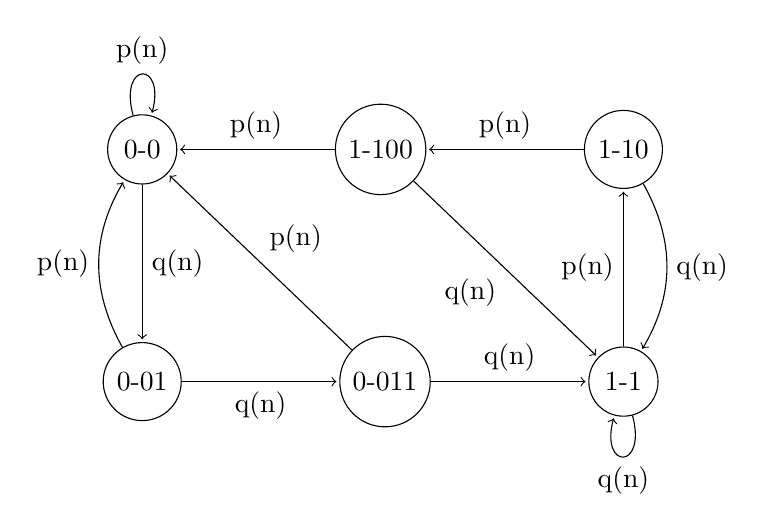
\begin{tikzpicture}
          \node[state] (0-0) {0-0};
          \node[state, right=2cm of 0-0] (1-100) {1-100};
          \node[state, right=2cm  of 1-100] (1-10) {1-10};
          \node[state, below= 2cm of 0-0] (0-01) {0-01};
          \node[state, right= 2cm  of 0-01] (0-011) {0-011};
          \node[state, right=  2cm of 0-011] (1-1) {1-1};
          \draw[every loop]
              (0-0) edge[auto=left] node {q(n)} (0-01)
              (0-01) edge[bend left, auto=left] node {p(n)}(0-0)
              (0-0) edge[loop above] node{p(n)} (0-0)
              (0-01) edge[auto=right] node{q(n)} (0-011)
              (0-011) edge[auto=right] node{p(n)} (0-0)
              (0-011) edge[auto=left] node{q(n)} (1-1)
              (1-1) edge[loop below] node{q(n)} (1-1)
              (1-1) edge[auto=left] node{p(n)} (1-10)
              (1-10) edge[bend left, auto=left] node{q(n)} (1-1)
              (1-10) edge[auto =right] node{p(n)} (1-100)
              (1-100) edge[auto=right] node{q(n)} (1-1)
              (1-100) edge[auto=right] node{p(n)} (0-0);
       \end{tikzpicture}
   \end{center}
    \\
    where \\
   p(n)= Probability of occurrence of 0 \\
   q(n) = Probability of occurrence of 1
   \end{block}
\end{frame}

\begin{frame}
\frametitle{Steady State Probabilities}
\begin{itemize}
\item Now we will study the asymptotic behaviour of the solution of the above system in the time-homogeneous case, i.e., in the case that the functions p(n) and q(n) are constant. For such p(n) and q(n) we are able to determine the limits ( so called steady-state probabilities) \\
\[\lim_{n\to\infty}p(n) \hspace{0.5cm}and \hspace{0.2cm} \lim_{n\to\infty}q(n) \]
\end{itemize}
  \begin{theorem}
    Suppose that function p(n) and q(n) are constant, p\equiv p \in (0 1) and q \equiv q=1-p.Then \\
    \[\lim_{n\to\infty}x(n)=\frac{p^{w-1}(1-q^w)}{p^{w-1}(1-q^w)+q^{w-1}(1-p^w)}\]
    \[\lim_{n\to\infty}y(n)=\frac{q^{w-1}(1-p^w)}{p^{w-1}(1-q^w)+q^{w-1}(1-p^w)}\]
    where w = length of the string of 0's and 1's
    
  \end{theorem}
    
\end{frame}    
\begin{frame}
  \begin{proof}
  First, we compute the limits of the auxiliary functions \(a_j\) , j = 1,..., 2w.
  We will denote them as
  \[\pi_j=\lim_{n\to\infty}a_j(n), \hspace{0.2cm}j=1,2,3,4,...2w\]
  \[\boldsymbol{\pi}=(\pi_1,\pi_2,\pi_3,....\pi_{2w})\]
  The vector \boldsymbol{\pi} is the solution of the system :
  \[\boldsymbol{\pi}=\boldsymbol{\pi P}\]
  with the condition that :
  \[\sum_{j=1}^{2w}\ \pi_j=1\]
  where \textbf{P} is the transition matrix.
  \end{proof}    
\end{frame}
\begin{frame}
  \begin{block}{Continue..}
    Since 
    \[x(n)=\sum_{j=1}^{w}a_j(n) \hspace{0.2cm} and \hspace{0.2cm} y(n)=\sum_{j=w+1}^{2w}a_j(n)\]
    \hspace{2cm}\Rightarrow \\ 
    \[\lim_{n\to\infty}x(n)=\sum_{j=1}^{w}a_j(n) \hspace{0.2cm} and \hspace{0.2cm} \lim_{n\to\infty}y(n)=\sum_{j=w+1}^{2w}a_j(n)\]
    For simlicity I am considering w=3 \\
    Since 
    \begin{align}
        \boldsymbol{\pi(n+1)} &= \boldsymbol{\pi(n) P} \nonumber
    \end{align}
    In the limiting case \[\boldsymbol{\pi(n+1)}=\boldsymbol{\pi(n)}=\boldsymbol{\pi}\]
    So
  \end{block}
    
\end{frame}
\begin{frame}
   \begin{block}{continue}
   \begin{align}
       \boldsymbol{\pi} &= \boldsymbol{\pi P} \nonumber \\
       \boldsymbol{\pi}^T &= (\boldsymbol{\pi P})^T \nonumber \\
       \boldsymbol{\pi}^T &= \boldsymbol{P}^T\boldsymbol{\pi}^T \nonumber \\
       (\boldsymbol{P}^T-\boldsymbol{I})\boldsymbol{\pi}^T &= \boldsymbol{o} \nonumber  \\
       \boldsymbol{P}^T-\boldsymbol{I}&=\begin{pmatrix}
                                         p-1 & p & p & 0 & 0 & p \\
                                         q  & -1 & 0 & 0 & 0 & 0 \\
                                         0 & q-1 & 0 & 0 & 0 & 0 \\
                                         0 & 0   & q & q-1 & q & q \\
                                         0 & 0 & 0 & p & -1 & 0 \\
                                         0 & 0 & 0 & 0 & p & -1 
                                         \end{pmatrix} \nonumber 
   \end{align}
    
   \end{block}
    
\end{frame}
\begin{frame}
  \begin{block}{Continue...}
  \begin{align}
      \boldsymbol{P}^T-\boldsymbol{I}& \sim \begin{pmatrix}
                                            -q & p & p & 0 & 0 & p \\
                                            0 & -q & p & 0 & 0 & p \\
                                            0 & 0 & -q & 0 & 0 & p \\
                                            0 & 0 & 0 & -p & q & 1 \\
                                            0 & 0 & 0 & 0 & -p & 1 \\
                                            0 & 0 & 0 & 0 & 0 & 0
                                            \end{pmatrix} \nonumber
  \end{align}
  the rank of the above matrix is 5=2w-1 for w=3 and we have another equation :
  \[\sum_{j=1}^{2w}\pi_j = 1\]
  Hence the above system has the unique solution.
  \end{block}
    
\end{frame}    
\begin{frame}
  \begin{block}{Continue..}
    \[\pi_5=\frac{\pi_6}{p}\]
    \[\pi_4=\frac{\pi_5}{p}=\frac{\pi_6}{p^2}\]
    \[\pi_3=\frac{p}{q}\pi_6\]
    \[\pi_2=\frac{1}{q}\pi_3=\frac{p}{q^2}\pi_6\]
    \[\pi_1=\frac{1}{q}\pi_2=\frac{p}{q^3}\pi_6\]
    Since 
    \[\pi_1+\pi_2+\pi_3+\pi_4+\pi_5+\pi_6=1\]
    \[\pi_6\left(\frac{p}{q^3}+\frac{p}{q^2}+\frac{p}{q}+\frac{1}{p^2}+\frac{1}{p}+1\right)=1\]
   \end{block}  
   
\end{frame}
\begin{frame}
  \begin{block}{Continue...}
  \begin{align}
      \pi_6 & =\frac{p^2q^3}{p^3(1+q+q^2)+q^3(1+p+p^2)} \nonumber \\
      \lim_{n\to\infty}x(n) &= \pi_1+\pi_2+\pi_3 \nonumber \\
                            &=\frac{p}{q^3}\pi_6+\frac{p}{q^2}\pi_6+\frac{p}{q}\pi_6 \nonumber \\ &=\left(\frac{p}{q^3}+\frac{p}{q^2}+\frac{p}{q}\right)\pi_6 \nonumber  \\
                            &=\left(\frac{p+pq+pq^2}{q^3}\right)\left(\frac{p^2q^3}{p^3(1+q+q^2)+q^3(1+p+p^2)}\right) \nonumber \\
                            &=\frac{p^2(1-q^3)}{p^2(1-q^3)+q^2(1-q^3)} \nonumber
  \end{align}
  Similar expression can be obtained for \lim_{n\to\infty}y(n)
    
  \end{block}
    
\end{frame}
\begin{frame}
  \begin{block}{Further Research}
  \begin{itemize}
  \item When modelling the data and clock recovery, the functions
  p(n) and q(n) are not constant but they are periodic functions of the
  argument n.
  \item Investigation of the asymptotic properties of the solution in such case is a much more complicated task and will be subject to further research.
  \end{itemize}
  \end{block}
    
\end{frame}
    




\end{document}